\documentclass[handout]{beamer}
\usepackage[frenchb]{babel}
\usepackage[T1]{fontenc}
\usepackage[utf8]{inputenc}
\usepackage{graphicx}
\usepackage{subfig}

% functions to plot
\def\func(#1){(#1)*(1-(#1))}
\hypersetup{colorlinks = true,linkcolor = blue,urlcolor  = blue}
            
\newcommand{\qGraph}[1]{\begin{center} \includegraphics[width =
\textwidth]{#1}\end{center}}

\newcommand{\mcl}{\mathcal}

\addtobeamertemplate{navigation symbols}{}{%
    \usebeamerfont{footline}%
    \usebeamercolor[fg]{footline}%
    \hspace{1em}%
    \insertframenumber/\inserttotalframenumber
}

\newenvironment{iPar}[1]{\textbf{#1} \begin{itemize}}{\end{itemize}}

\newcommand{\inc}{{inc}}
\newcommand{\cp}{{cmp}}
\newcommand{\bull}{$\bullet\;$} 

\newcommand{\esp}{\mathbf{E}} \newcommand{\ul}[1]{\underline{#1}}
\newcommand{\ol}[1]{\overline{#1}} \newcommand{\ora}[1]{\textbf{#1}}
\newcommand{\wh}{\widehat}
\newcommand{\mdp}{\medskip \pause}
\newcommand{\mc}{\mathcal}

\title{Intertemporal Choice}
\author{Microeconomics \\ 20851}
\date{}

\begin{document}

\frame{\titlepage}

\section[Outline]{}
\frame{\tableofcontents}

\section{}


\begin{frame}\frametitle{Roadmap}

\begin{iPar}{Up until now}
\item Consumer choice
\item Price and income effects
\item Risk 
\end{iPar}\mdp

\begin{iPar}{This class: Intertemporal choice}
\item To understand savings and durable goods consumption
\end{iPar}\mdp

\begin{iPar}{Coming up}
\item  Measuring welfare and well-being 
\item  Market equilibrium in an exchange situation
\item  Production decisions in a firm
\item Strategic behaviour of firms
\item Auctions
\end{iPar}

\end{frame}

\section{Preferences}

\begin{frame}\frametitle{Preferences}

Individuals generally prefer to benefit in the present and to delay costs:

\begin{itemize}
\item Have a coffee right now vs. at the break?
\item Go to the gym today vs. tomorrow?
\item Saving today to consume once you retire?
\end{itemize}

\end{frame}


\begin{frame}\frametitle{Discounted utility}

If $u(C_t)$ is the utility gained from consumption at time $t$, the discounted utility for a consumption plan $\textbf{C} = (C_1,...,C_T)$ is :


$$ DU(\mathbf{C}) = \sum_{t=1}^T \delta^{t-1} u(C_t) $$

$\delta$ $\in [0,1]$ is the discount factor (patience) whereas $\mathbf{C} = (C_1,...,C_T)$. The relation between the discount factor, $\rho$ and $\delta$ is given by: 

$$ \delta = \frac{1}{1+\rho} $$

\end{frame}

\begin{frame}\frametitle{Marginal Rate of Substitution (MRS)}

If $T=2$, then $$ DU(\textbf{C}) = u(C_1) +  \delta u(C_2) $$. The total differential gives the MRS: 

$$ \frac{\partial C_2}{\partial C_1}\rvert_{dDU=0} = -\frac{u'(C_1)}{\delta u'(C_2)}$$

Intertemporal preferences are caracterized by: 

\begin{itemize}
\item The discount factor ($\delta$)
\item The shape of $u$. 
\end{itemize}

\textbf{Exercise A}: Find the MRS for $u(C_t) = \log C_t$

\end{frame}


\begin{frame}{How to Estimate Discount Rates?}

An Experiment in Denmark  (Harrison, Lau and Williams, 2002)

\begin{figure}
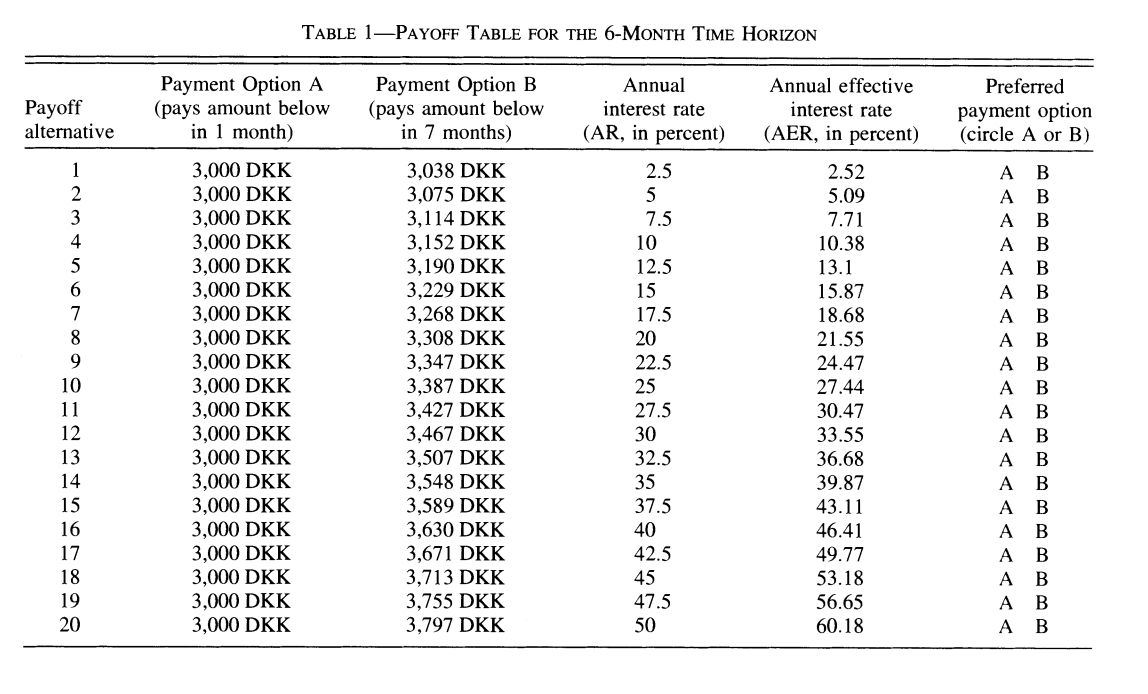
\includegraphics[scale=0.5]{MPL.png}
\end{figure}


\end{frame}

\begin{frame}{Results of Discount Rates}

Expérience au Danemark  (Harrison, Lau et Williams, 2002)

\begin{figure}
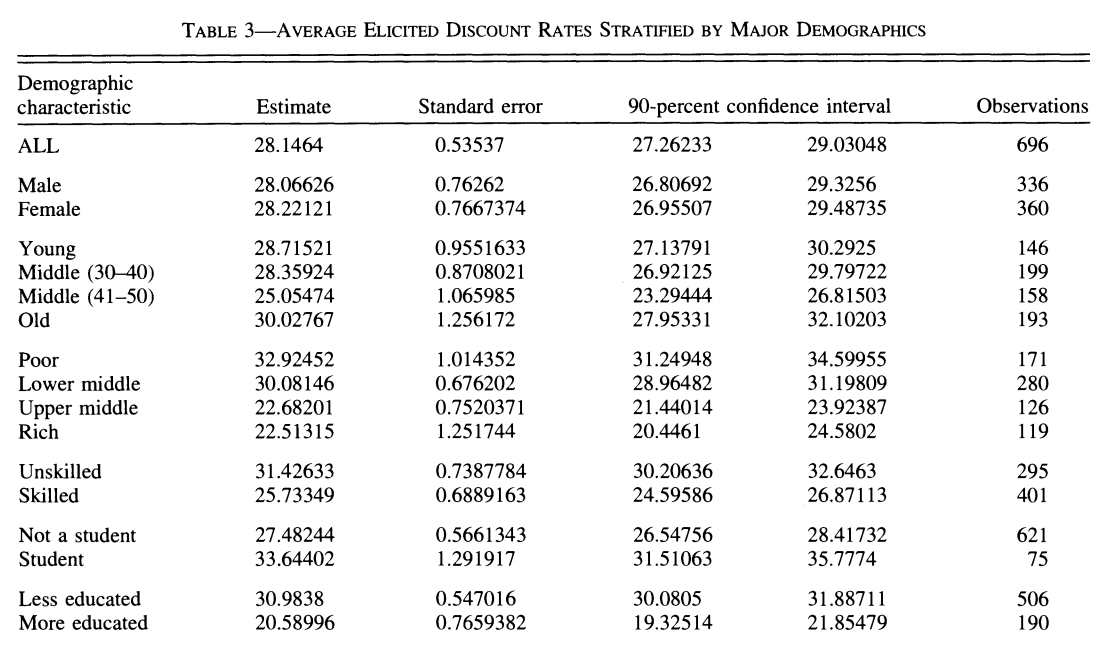
\includegraphics[scale=0.5]{Results.png}
\end{figure}

\end{frame}

\section{The Intertemporal Constraint}

\begin{frame}{Interest and Financial Markets}

Financial institutions offer us $r_S$ for every dollar we deposit (save). They also ask a compensation $r_D$ for each dollar lent

For now, let's suppose $r_D = r_S = r$. 

\end{frame}

\begin{frame}{Resources}

Resources come from two sources:
\begin{itemize}
\item initial wealth: $W_0$. 
\item income in both periods, $Y_1$, $Y_2$. 
\end{itemize}

The present value of resources is : 

$$ VP_W = W_0 + Y_1 + \frac{Y_2}{1+r} $$
 
\end{frame}

\begin{frame}{Constraint}

The present value of consumption for both periods is : 

$$VP_C = C_1 + \frac{C_2}{1+r}$$. 

Thus, the intertemporal constraint is $ VP_C \leq VP_W $:

$$ C_1 + \frac{C_2}{1+r} \leq W_0 + Y_1 + \frac{Y_2}{1+r}  $$

\end{frame}

\begin{frame}{Borrowing and Saving}

We can rewrite the constraint such that :

$$ (1+r)(W_0 + Y_1 - C_1) \ge  C_2 - Y_2 $$

Therefore,

\begin{itemize}
\item The individual that saves during the first period (LHS positive) can consume more than his income during the second period (positive RHS).
\item The individual that borrows during the first period (LHS negative) can consume less than his income during the second period (negative RHS).
\end{itemize}

\end{frame}


\begin{frame}{Visual}

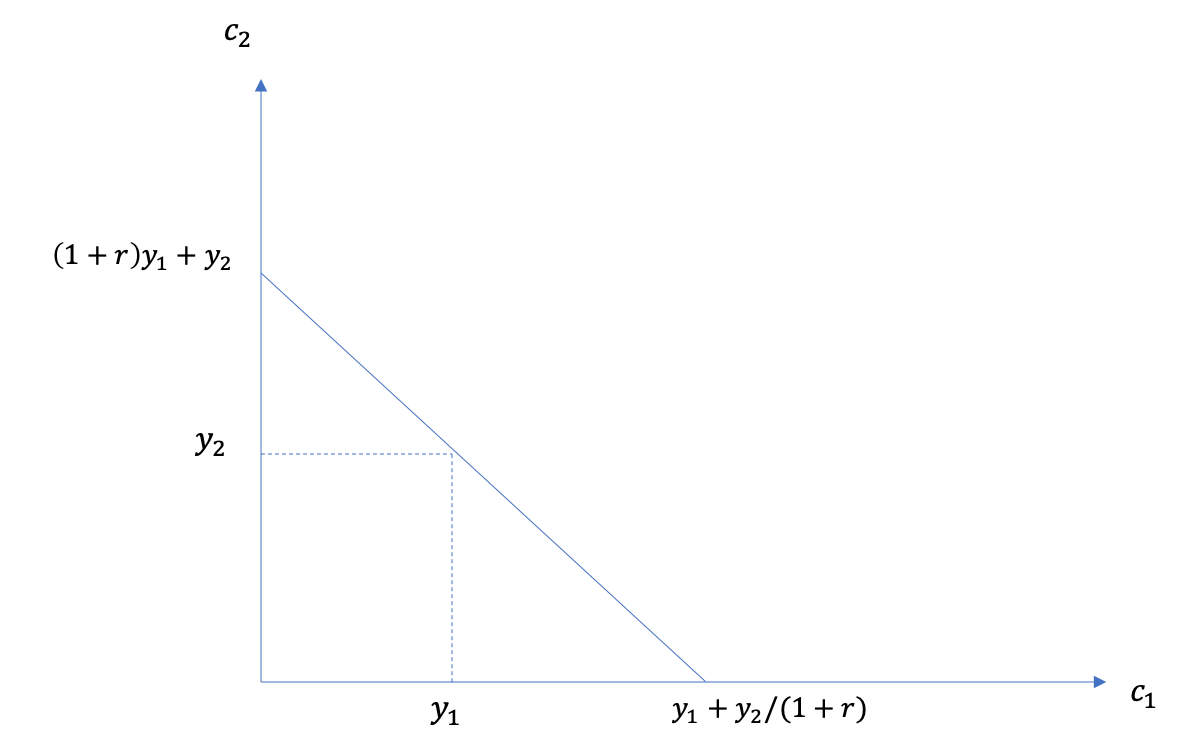
\includegraphics[scale=0.5]{budget.png}

\end{frame}


\begin{frame}{Example: Contributive Retirement Plan}

A defined benefit pension plan requires savings during the first period. 
\begin{itemize}

\item Income in the second period is $Y_2 = \phi Y_1$ with $\phi \in [0,1]$. 
\item Income in the first period is reduced by the contribution, $\tau Y_1$. 

\end{itemize}

The resource constraint is therefore: 

$$ C_1 + \frac{C_2}{1+r} \leq W_0 + (1-\tau)Y_1 + \frac{\phi Y_1}{1+r}  $$

The contribution rate $\tau$ is chosen by actuaries such that : 

$$ \tau Y_1 = \frac{\phi Y_1}{1+r_P} \to \tau = \frac{\phi}{1+r_P} $$

where $r_P$ is the yield of the pension plan. If $r_P = r$, the budget constraint does not change! consumption doesn't change when $\phi$ increases and savings will then adjust (Crowding out).

\end{frame}

\begin{frame}{Rate Differentials}

\textbf{Exercise B}: What will the constraint look like if $r_S<r_D$?

\textbf{Exercise C}: How do we represent a situation where an individual cannot borrow?

\end{frame}

\section{Optimal Choice}

\begin{frame}{Maximization}

The problem is (set $W_0=0$ to simplify):

$$ \max_{C_1,C_2} \{ u(C_1) + \delta u(C_2) : C_1+C_2/(1+r) \leq Y_1 + Y_2/(1+r)\}  $$

Two approaches: 
\begin{enumerate}
\item Direct approach (constraint substitution)
\item Lagrangian	
\end{enumerate}


\end{frame}

\begin{frame}{Optimality condition}

The lagrangian gives 3 FOC:

\begin{eqnarray}
 u'(C_1) - \lambda = 0  \\
\delta u'(C_2) - \lambda /(1+r) = 0  \\
C_1+C_2/(1+r) - Y_1 - Y_2/(1+r) = 0  
\end{eqnarray}

With (1) and (2) we find that : 

$$ \frac{u'(C_1)}{\delta u'(C_2)} = 1+r $$

By rearranging and setting $R=1+r$, we obtain Euler's equation: 
$$ u'(C_1) = R\delta u'(C_2) $$
\end{frame}

\begin{frame}{Visual}
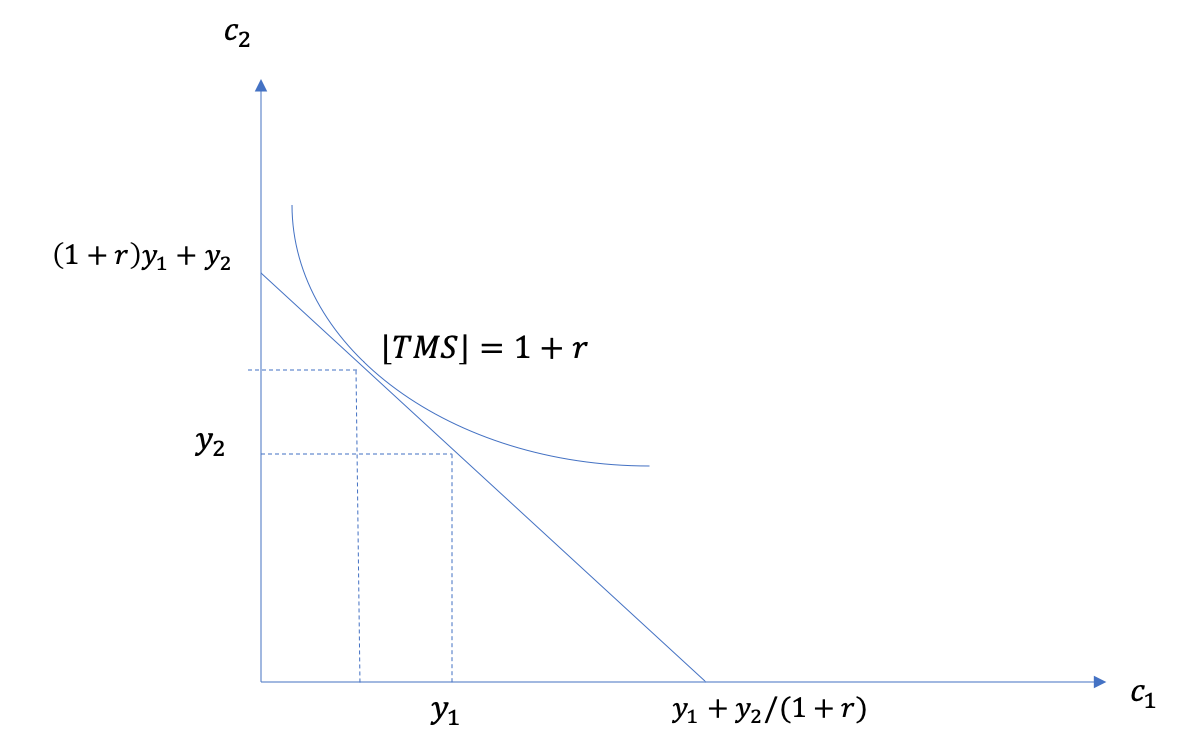
\includegraphics[scale=0.5]{optimal.png}
\end{frame}

\begin{frame}{Example}

\textbf{Exercise D}: Solve to find the optimal choice of $C_1$ and $C_2$ if $u(C)=\frac{C^{1-\sigma}}{1-\sigma}$

\end{frame}

\begin{frame}{Example: Are We Saving Enough?}

There is a lot of literature and an important public debate to determine whether people are saving enough for retirement.

\begin{figure}
	
\includegraphics[scale=0.4]{retraite.png} 
	\caption{Le Conseiller, Globe and Mail, L'Actualité}
\end{figure}

\end{frame}

\begin{frame}{Replacement Rate}

\begin{figure}
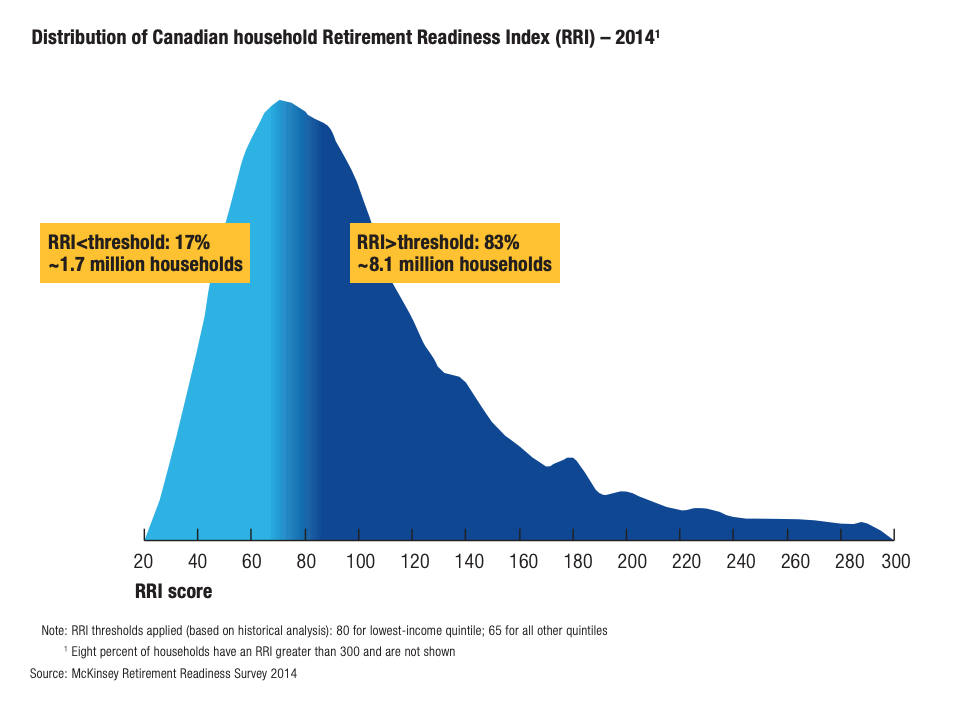
\includegraphics[scale=0.4]{mckinsey.png} 
\caption{McKinsey (2015)}
\end{figure}
	
\end{frame}

\begin{frame}{Optimal Saving Level}

What does theory say about how much people should save?\vspace{0.25in}

\textbf{Exercise E}: Find an expression for the optimal savings level at the beginning of period 2 if $u(C)=\frac{C^{1-\sigma}}{1-\sigma}$ and the constraint is given by:

$$ C_1 + \frac{C_2}{1+r} \leq (1-\tau)Y_1 + \frac{\phi Y_1}{1+r}  $$ 

\end{frame}


\begin{frame}{Example: Are We Saving Enough?}

We can take into account preferences by simulating how much people should be saving (and comparing it to reality).

\begin{figure}
	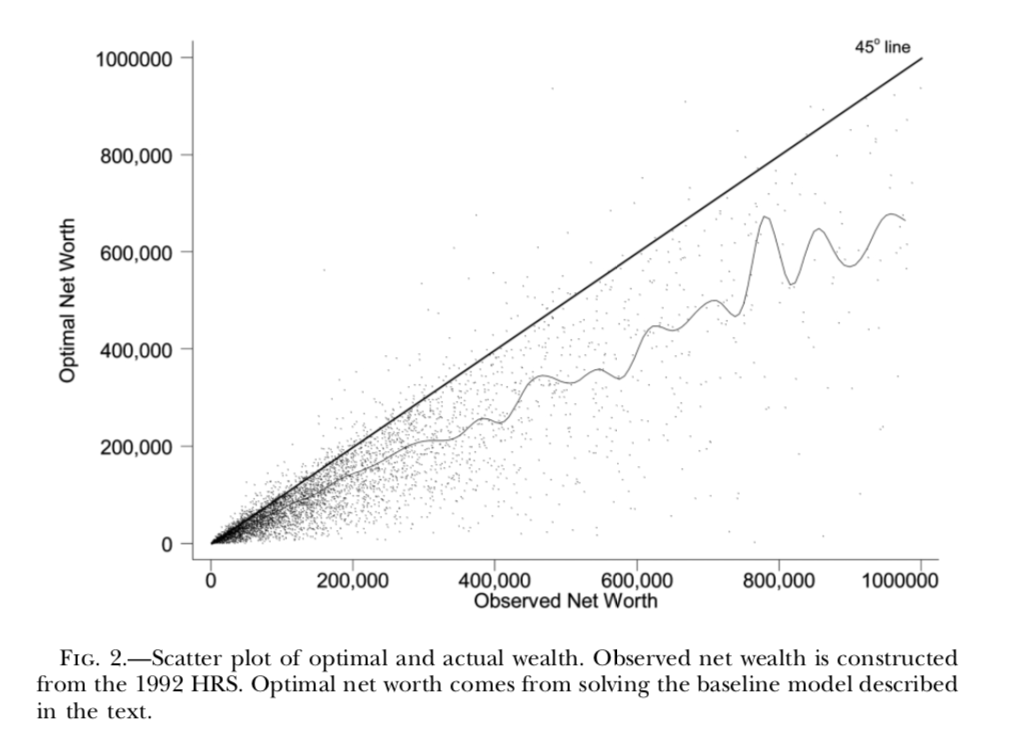
\includegraphics[scale=0.4]{savings.png}
	\caption{Scholz et al. (2007, Journal of Political Economy)}
\end{figure}


\end{frame}

\section{Bias towards the present}

\begin{frame}{Present-bias: Choosing a movie}

You have to choose a movie to watch tonight and a movie that you will watch next week: 

\begin{figure}
\subfloat[Mommy (Xavier Dolan)]{
\includegraphics[scale=0.5]{Mommy.png}}
\subfloat[Les Boys (Louis Saia)]{
\includegraphics[scale=0.5]{boys.png}}

\end{figure}

\end{frame}

\begin{frame}{Preference Bias - The Present}

Suppose that "Mommy" has an immediate benefit of 4 and a future benefit of 4 but that "Les Boys" has an immediate benefit of 7 (no future benefit). \vspace{0.25in}

\textbf{Exercise F}: What is the discounted utility if you're choosing for today and $\delta=1$. What if you're choosing for next week?

\end{frame}


\begin{frame}{Preference Bias - The Present}

Laibson (1997) suggests the quasi-hyperbolic discounted utility: 

$$QH(\mathbf{c}) = u(C_1) + \beta \sum_{t=2}^T \delta^{t-1} u(C_t)$$

\textbf{Exercise G}: What is the MRS between consumptions $C_1$ and $C_2$? And $C_2$ vs. $C_3$? Compare with the expected utility.

\end{frame}

\begin{frame}{Preference Bias - The Present}

Using these two movies, suppose $\beta=0.5$. 
\vspace{0.5in}

\textbf{Exercise H}: Which film would you choose for today with preferences biased towards the present? What about choosing for next week?

\end{frame}

\begin{frame}{Example: Why Buy a Gym Membership?}

A single-use pass costs 10\$. The cost per visit of people buying a membership is far higher than 10\$. 

\begin{figure}
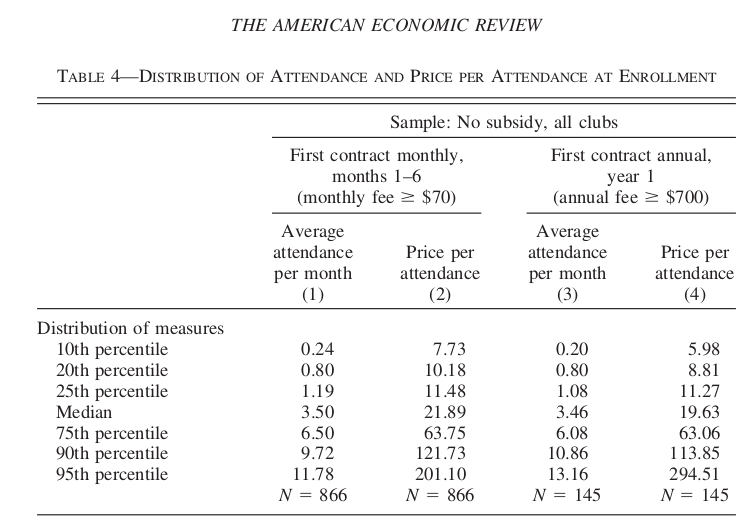
\includegraphics[scale=0.3]{Gym.png}
\caption{Della Vigna et Malmendier (2006)}
\end{figure}

\end{frame}

\begin{frame}{Example: How Can We Help People Save?}

\begin{itemize}
\item Saving is like exercising: costly in the short run, beneficial in the long run.
\item We could decide to change the default option (a well-known mechanism in psychology): opt-in vs. opt-out (nudges, related to prospect theory)
\item Shea et Madrian (2001, QJE) show that savings go up significantly in the short run within firms using the opt-out default option
\end{itemize}

\end{frame}

\begin{frame}{The Power of Nudges}
Participation increases significantly among new employees.
	\begin{figure}
		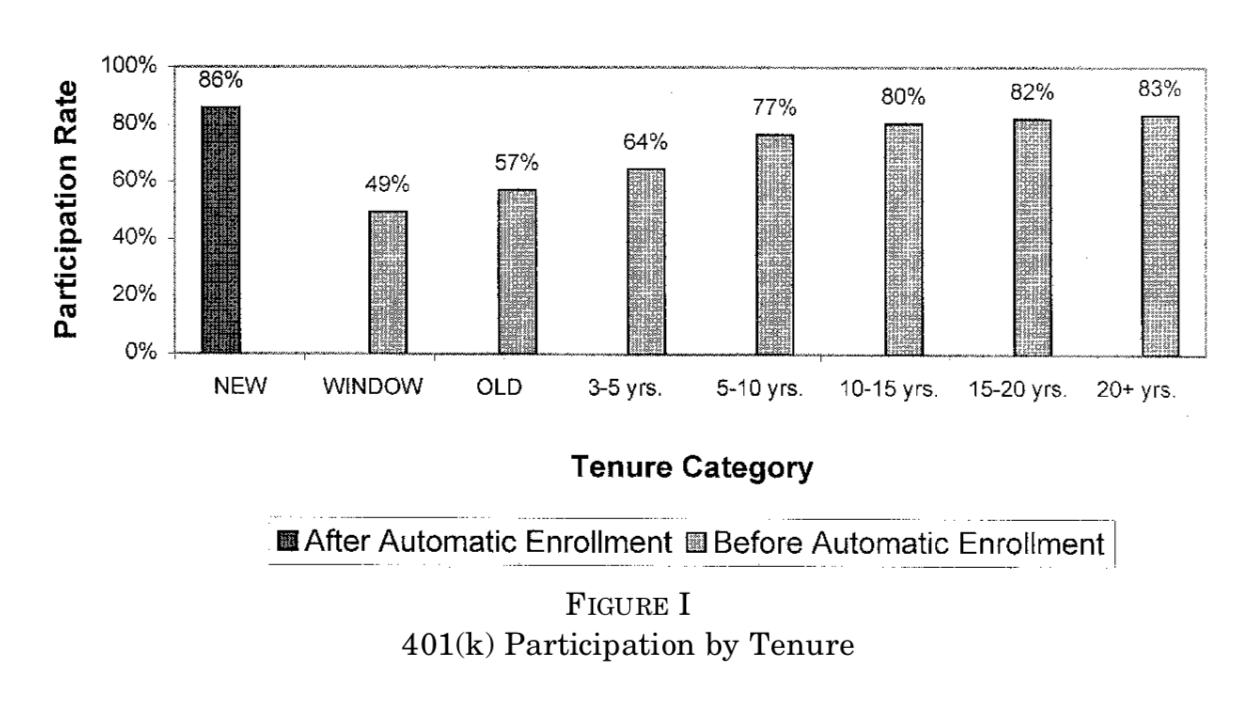
\includegraphics[scale=0.45]{shea.png}
		\caption{Shea et Madrian (2001, QJE)}
	\end{figure}
\end{frame}


\end{document}




